%%%%%%%%%%%%%%%%%%%%%%%%%%%%%%%%%%%%%%%%%%%%%%%%%%%%%%%%%%%%%%%%%%%%%%%
% Project Name : HyperPath                                            %
% Project Home : https://github.com/TeamAC/HyperPath                  %
% Part         : Bibliography                                         %
% Author       : chedi                                                %
% Comments     :                                                      %
%                                                                     %
%%%%%%%%%%%%%%%%%%%%%%%%%%%%%%%%%%%%%%%%%%%%%%%%%%%%%%%%%%%%%%%%%%%%%%%

\section{Data model}

\section{EJB Server Bean}

\subsection{Annotations}
\subsubsection{Introduction}
Annotation is a simple, expressive means of decorating Java source code with metadata that is compiled into the corresponding Java class files for interpretation at run time by a JPA persistence provider to manage persistent behavior.

A metadata annotation represents a Java language feature that lets you attach structured and typed metadata to the source code. Standard JPA annotations are in the javax.persistence package.

\subsubsection{Advantages and Disadvantages of Using Annotations}
Using annotations provides several advantages:
\begin{itemize}
\item They are relatively simple to use and understand.
\item They provide in-line metadata within with the code that it describes; you do not need to replicate the source code context of where the metadata applies.
\end{itemize}

The primary disadvantage of annotations is that the metatdata becomes unnecessarily coupled to the code. changes to metadata require changing the source code.

\subsection{Abstraction of data access}
Mapping relational databases to objects is a well-understood task by now, thus there are plenty of supporting tools, and normally those tools generate code. Eclipse itself comes with a tool to create entities from tables, so do other IDEs and of course the major UML tools can do that as well.

On the other hand, when you access the database via JPA, you either ask the EntityManager for entities that you have an id for, or you create query objects, execute them and get lists of objects as results. If you use queries (which we do), you express them in the Java Persistence Query Language.

\subsection{Using EclipseLink JPA Extensions for Mapping}
The Java Persistence API (JPA), part of the Java Enterprise Edition 5 (Java EE 5) EJB 3.0 specification, greatly simplifies Java persistence and provides an object relational mapping approach that allows you to declaratively define how to map Java objects to relational database tables in a standard, portable way that works both inside a Java EE 5 application server and outside an EJB container in a Java Standard Edition (Java SE) 5 application.

EclipseLink persistence provider applies the first annotation that it finds; it ignores other mapping annotations, if specified. If EclipseLink persistence provider does not find any of the mapping annotations from the preceding list, it applies the defaults defined by the JPA specification: not necessarily the @Basic annotation.

Here we use various annotation to configure the persistent behavior of your entities:
\begin{lstlisting}[label=Emails JPA entity,caption=Emails JPA entity]
@Entity
@XmlRootElement

@Table(
  name    = "emails",
  schema  = "",
  catalog = "hyperPath",

  uniqueConstraints = {
    @UniqueConstraint(columnNames = {"address"})
  })

@NamedQueries({
  @NamedQuery(
    name  = "Emails.findAll",
    query = "SELECT e FROM Emails e"),
  @NamedQuery(
    name  = "Emails.findById",
    query = "SELECT e FROM Emails e WHERE e.id = :id"),
  @NamedQuery(
    name  = "Emails.findByAddress",
    query = "SELECT e FROM Emails e WHERE e.address = :address")
})

public class Emails implements Serializable {
  private static final long serialVersionUID = 1L;
  @Id
  @NotNull
  @Basic(optional = false)
  @Column(name = "id", nullable = false)
  @GeneratedValue(strategy = GenerationType.IDENTITY)
  private Integer id;

  @NotNull
  @Basic(optional = false)
  @Size(min = 1, max = 100)
  @Column(name = "address", nullable = false, length = 100)
  private String address;

  @ManyToMany(mappedBy = "emailsList")
  private List<Entities> entitiesList;

   /**
    * Rest of the Email entity class (POJO) See Emails.java
  	* .......
  	*/
}
\end{lstlisting}

\subsection{JPA Persistence Unit}
A persistence unit configures various details that are required when you acquire an entity manager. You specify a persistence unit by name when you acquire an entity manager factory. You configure persistence units in JPA persistence descriptor file \textbf{\textit{\textsf{persistence.xml}}}.

In this file, you can specify the vendor extensions that this reference describes by using a \textit{\textbf{\textsf{<properties>}}} element.

\begin{lstlisting}[label=Persistence unit persistence.xml,caption=Persistence unit persistence.xml]
<?xml version="1.0" encoding="UTF-8"?>

<persistence version="2.0"
  xmlns="http://java.sun.com/xml/ns/persistence"
  xmlns:xsi="http://www.w3.org/2001/XMLSchema-instance"
  xsi:schemaLocation="http://java.sun.com/xml/ns/persistence
  http://java.sun.com/xml/ns/persistence/persistence_2_0.xsd">

  <persistence-unit
    name="HyperPathServerPU"
    transaction-type="JTA">
    <provider>
      org.eclipse.persistence.jpa.PersistenceProvider
    </provider>

    <jta-data-source>
      jdbc/HyperPathData
    </jta-data-source>

    <exclude-unlisted-classes>
      false
    </exclude-unlisted-classes>

    <properties>
      <property
        name="eclipselink.ddl-generation"
        value="create-tables"/>
    </properties>

  </persistence-unit>
</persistence>
\end{lstlisting}

\footnote{Avoiding Clear text Passwords: EclipseLink does not support storing encrypted passwords in the persistence.xml file. For a Java EE application, you do not need to specify your password in the persistence.xml file. Instead, you can specify a data-source. This datasource is specified on the application server, and can encrypt the your password with its own mechanism.
}

\subsection{Calling the bean as a SOAP web service}
There is an easy way to access Service Beans: we simply annotate their class as web service. If we don’t care about the exact schema of the WDSL that gets generated, it is enough to use one simple annotation like this:

\begin{lstlisting}[label=WebService Bean,caption=WebService Bean]
@WebService(serviceName = "EmailsServices")
@Stateless()
public class EmailsServices {
  @Resource
  private UserTransaction utx;

  @PersistenceUnit
  EntityManagerFactory emf;

  /**
   * List all emails
   */
  @WebMethod(operationName = "listAllEmails")
  public List<Emails> listAllEmails() throws
    Exception,
    NonexistentEntityException,
    RollbackFailureException
  {
    emf = Persistence.createEntityManagerFactory("HyperPathServerPU");
    EmailsJpaController controller = new EmailsJpaController(utx, emf);
    return controller.findEmailsEntities();
  }

  /**
   * Other web services, see EmailsServices.java
   * .....
   */
}
\end{lstlisting}

\pagebreak
\begin{landscape}
  \begin{figure}
    \begin{center}
      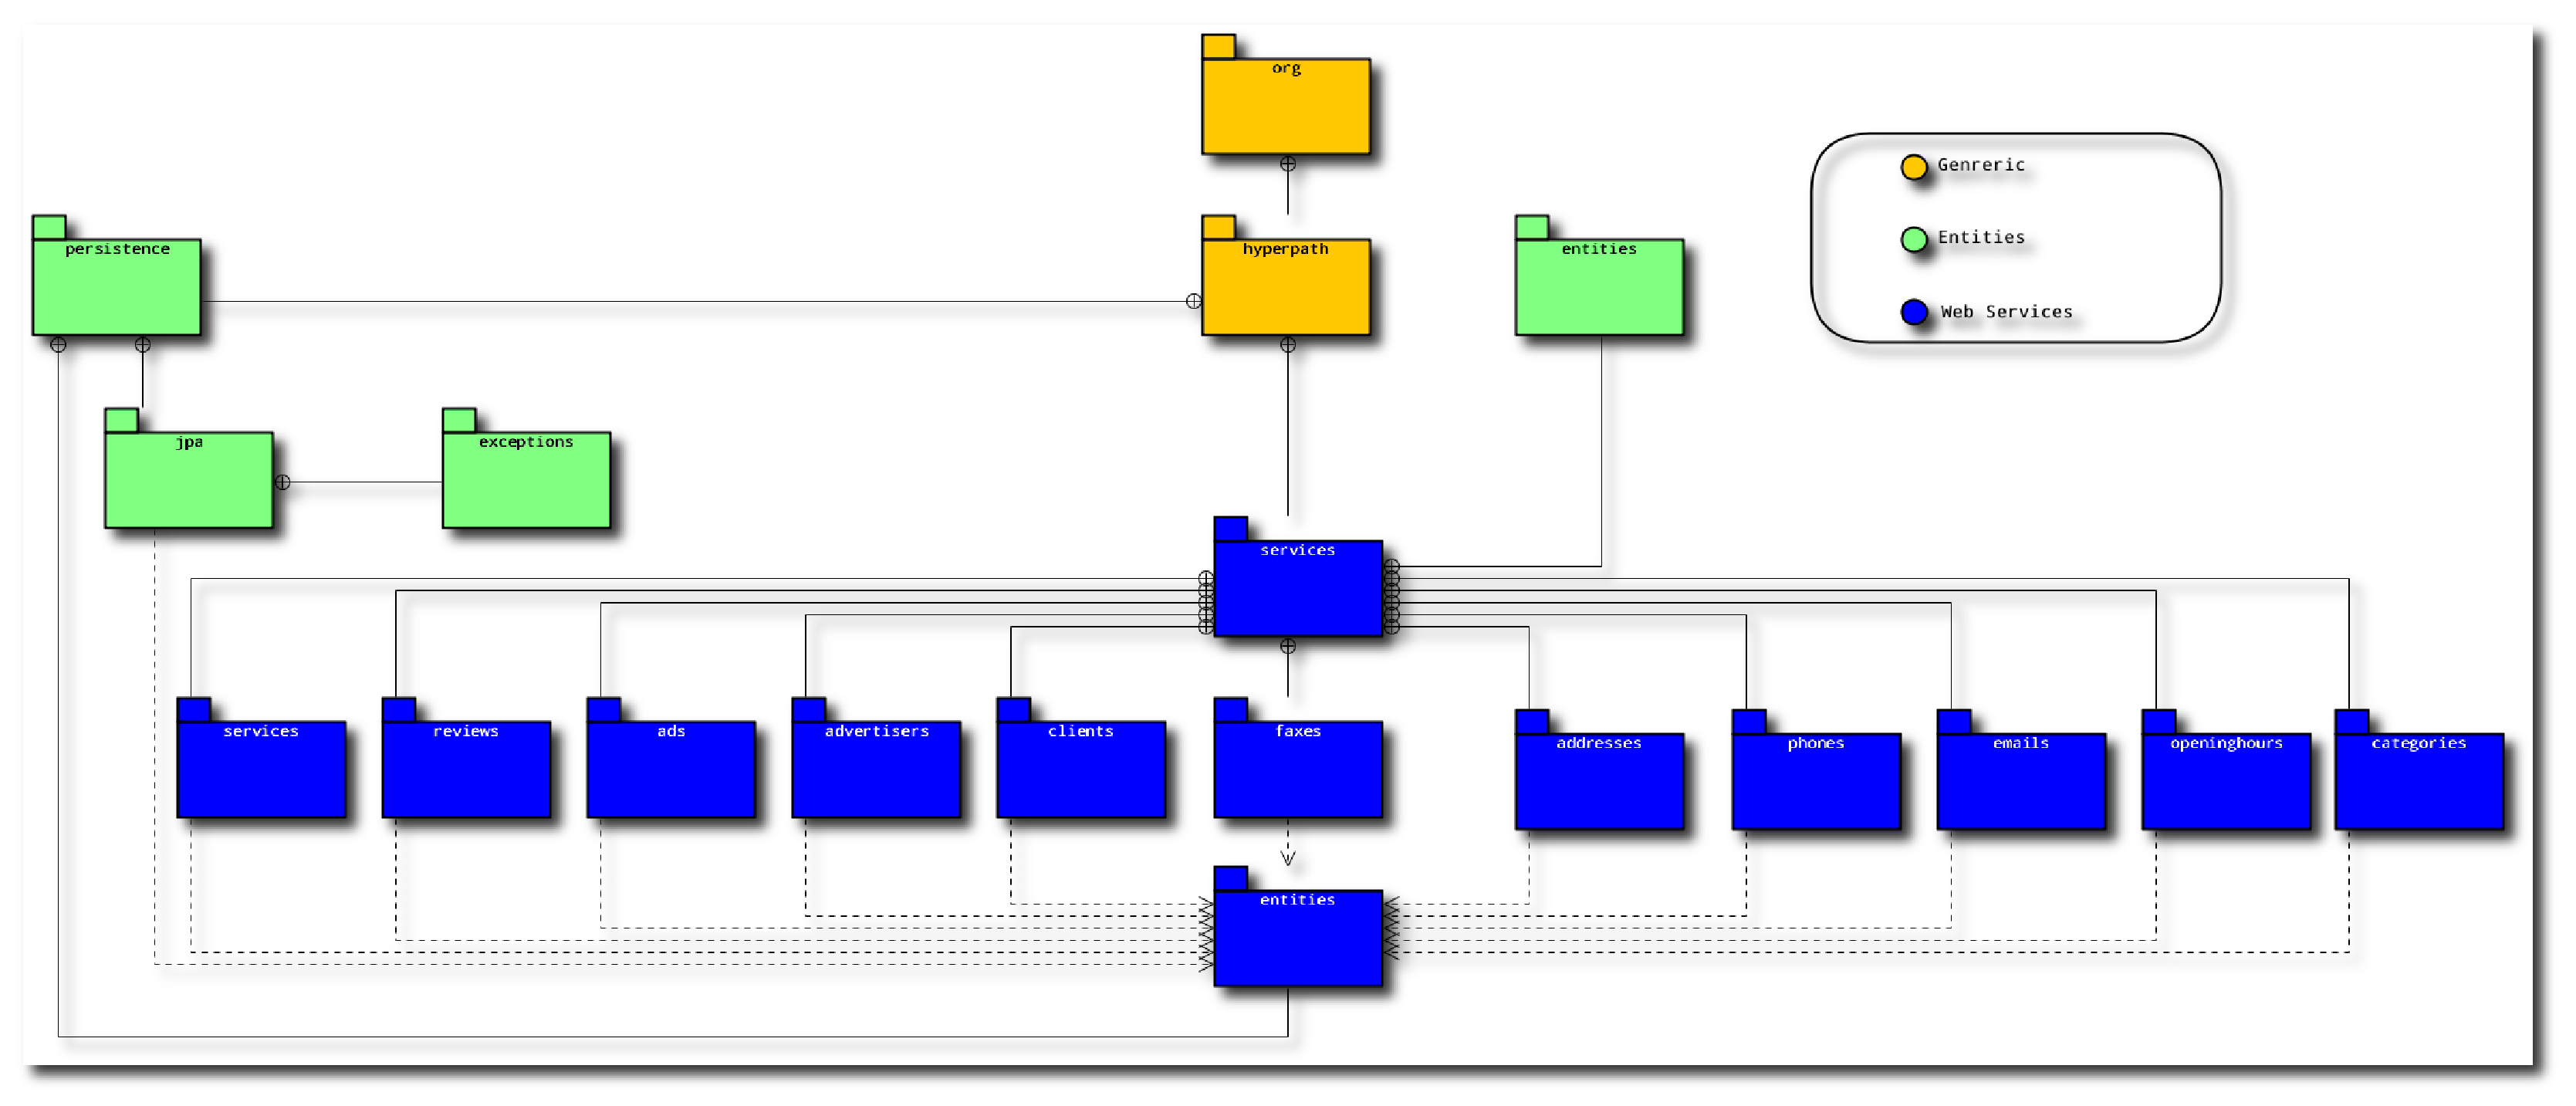
\includegraphics[scale=0.4]{Figures/HyperPath_server_packages.eps}
     \end{center}
     \caption{Server package architecture}
    \label{Server package architecture}
  \end{figure}
\end{landscape}